\documentclass[../main.tex]{subfiles}
\begin{document}
\part*{Project Background}
Image classification, also known as computer vision, is a field of study in artificial intelligence that involves training computer systems to identify, interpret, and understand images or visual data. It involves categorizing images into predefined classes or labels using machine learning algorithms. This process is similar to image recognition, which also uses machine learning algorithms to analyze and interpret visual data. Image recognition identifies and labels objects within an image, whereas image classification categorizes entire images.

% Image classification and image recognition are both computer vision tasks that involve analyzing and categorizing images. Both tasks use machine learning algorithms to analyze and interpret visual data. In image classification, an algorithm is trained to categorize images into predefined classes or labels, while in image recognition, an algorithm is trained to identify and label objects within an image. Although these tasks are distinct, they share many similarities and are often used in conjunction with each other. For example, image classification can be used as a preprocessing step for image recognition by categorizing images into relevant classes before identifying objects within them.

\begin{figure}[h!]
\centering
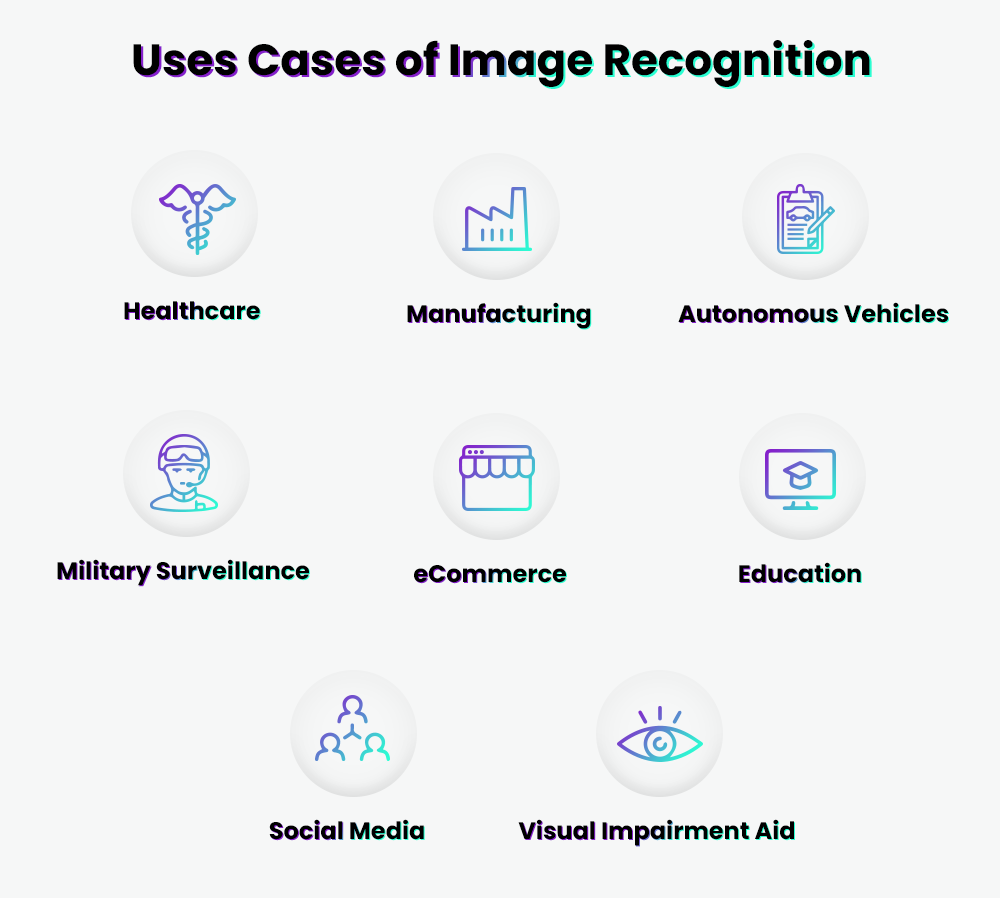
\includegraphics[scale=0.4]{images/image_rec_uses.png}
\caption{Some use-cases of Image Recognition.\citet{im}}
\label{fig:im_uses}
\end{figure}

Image classification, like image recognition, also has a wide range of applications across various industries such as healthcare, automotive, retail, security, and entertainment as shown in the Figure~\ref{fig:im_uses}. Image classification technology can be used for various tasks such as object detection, medical diagnosis, and product recognition. Some examples include:
\begin{itemize}
\item \textbf{Medical Diagnosis:} Image classification can be used for medical imaging analysis, identifying and diagnosing diseases like cancer, or detecting anomalies in medical images.
\item \textbf{Agriculture:} Image classification can be used for crop and soil analysis, plant disease detection, and monitoring crop growth and health.
\item \textbf{Manufacturing:} Image classification can be used for product quality control, identifying defects, and ensuring consistency in production lines.
\item \textbf{Retail:} Image classification can be used for product recognition, inventory management, and customer behavior analysis, such as tracking the popularity of certain products.
\item \textbf{Security:} Image classification can be used for object detection, facial recognition, and surveillance monitoring, such as identifying security threats and detecting suspicious behavior.
\item \textbf{Environmental Monitoring:} Image classification can be used for land use and land cover mapping, identifying deforestation or other changes in the environment, and monitoring wildlife populations.
\end{itemize}

\textbf{IaaS} (Infrastructure as a Service) is a cloud computing model in which cloud service providers offer virtualized computing resources such as servers, storage, and networking to users on a pay-per-use basis. IaaS allows users to scale up or down their computing resources as needed, without having to invest in their own infrastructure. Examples of IaaS providers include Amazon Web Services, Microsoft Azure, and Google Cloud Platform.

IaaS services have a wide range of applications across various industries, such as:
\begin{itemize}
    \item \textbf{Web hosting}: IaaS providers can host websites and web applications in the cloud, providing scalable and reliable infrastructure.
    \item \textbf{Big data}: IaaS providers can provide the computing resources needed to process and analyze large volumes of data.
    \item \textbf{Disaster recovery}: IaaS providers can provide backup and recovery solutions in the event of a disaster or outage.
    \item \textbf{DevOps}: IaaS providers can provide the infrastructure needed for software development and testing.
    \item \textbf{Machine learning}: IaaS providers can provide the computing resources needed to train and run machine learning models.
\end{itemize}





\end{document}

\clearpage